\section{Empirical Evaluation}\label{app:exps}
In this section, we thoroughly compare our method against the baselines mentioned in \Cref{table:compare}. We begin with a synthetic regression experiment in \Cref{app:data_generation}, in which the synthetic design allows us to control the heterogeneity in the data. This is followed in \Cref{app:acs} by another experiment on a real-world group-structured regression task drawn from the American Community Survey (ACS). 

\subsection{Synthetic Heterogeneous Regression Construction}
\label{app:data_generation}

We construct synthetic group-structured regression problems designed to test optimization under severe group heterogeneity. The data consist of $m$ groups. Each group $i$ has its own design matrix $\mA_{S_i}$ and target vector $\vb_{S_i}$, and defines a quadratic loss
\[
\ell_i(x) = \frac{1}{n_i} \|\mA_{S_i} \vx - \vb_{S_i}\|_2^2 \enspace.
\]
The objective of interest is the worst-group loss (as in \eqref{eq:main_objective})
\[
F(x) = \max_{i \in [m]} \ell_i(\vx) \enspace.
\]

We generate two qualitatively distinct group types to separate average performance from worst-group performance. The majority of groups are benign and geometrically aligned, whereas a small number have very high curvature, are geometrically misaligned, and are far from the population center. This construction ensures that minimizing the average loss does not coincide with minimizing the worst-group loss, and that curvature heterogeneity strongly affects optimization behavior.


We construct all group covariances relative to a shared orthonormal coordinate system. This allows us to control curvature direction-by-direction while keeping the ambient geometry comparable across groups. Each group, therefore, has a quadratic loss whose Hessian shares eigenvectors with the others but whose eigenvalues vary across groups.

\paragraph{Normal groups.}
Most groups are generated with a moderate condition number. Their Hessians have eigenvalues that vary across coordinates but remain within a controlled range. The corresponding optimal parameters are sampled from a distribution concentrated around a common center in parameter space. Independent noise is added to each group so that these losses are smooth and moderately curved. As a result, normal groups are geometrically aligned: their curvature structure is similar, and their optima lie in a relatively small region of parameter space.

\paragraph{Outlier groups.}
A small subset of groups is constructed to be adversarial in two distinct ways. First, each adversarial group has one direction with extremely large curvature, while the remaining directions retain moderate curvature. These sharp directions differ across adversarial groups. Second, the optimal parameter of each adversarial group lies far from the population center along its corresponding high-curvature direction. In addition, the noise level in these groups is set to be very small, so their losses are sharply concentrated around their optima. Together, these properties ensure that deviations along the sharp directions incur very large increases in the worst-group loss.

\paragraph{Implications of our construction.}
This construction produces three key phenomena:

\begin{enumerate}
    \item The stacked design matrix has a large condition number.
    \item The curvature directions that dominate different groups are misaligned.
    \item The empirical risk minimizer (which minimizes the average loss) can perform well on most groups while incurring substantial loss on a small number of adversarial groups.
\end{enumerate}

Because most groups share similar geometry, gradient averaging implicitly emphasizes their curvature structure. Therefore, first-order methods, reduce the average loss efficiently but make comparatively slow progress along the sharp directions that control the worst-group objective. In contrast, methods that adapt to local curvature or explicitly control worst-case behavior can continue to decrease the max-loss objective.

For the default instance used in \Cref{fig:iteration_runtime}, the problem dimension is $d=10$ with $100$ groups, of which $5$ are adversarial. The stacked Gram matrix has a condition number on the order of $10^5$, and the empirical risk minimizer exhibits a clear gap relative to the robust optimum computed via convex programming. For more details on data generation, see the included Jupyter notebook.

\subsubsection{Computing the Robust Optimum via Convex Programming}
To obtain a reliable reference point for evaluation, we compute the exact optimum value of the worst-group objective using a convex solver. Concretely, we solve the robust regression problem that minimizes the maximum group mean-squared error. Although the objective is a pointwise maximum over groups, it remains a convex function of the parameter vector because each group loss is a convex quadratic.

We programmatically formulate this problem using the epigraph trick. We introduce an auxiliary scalar variable $t$ that upper-bounds every group loss, and then minimize this upper bound. If we write the group loss as the mean squared residual for that group, then the epigraph reformulation becomes
\[
\min_{x,\, t}\ \ t
\quad\text{subject to}\quad
\ell_i(\vx) \le t
\ \ \text{for every group } i\in[m]\enspace.
\]
Each constraint is a convex quadratic inequality, so the resulting problem is a convex quadratically constrained program. We implement this formulation in \texttt{CVXPY}~\citep{diamond2016cvxpy,agrawal2018rewriting} by declaring decision variables for the model parameters and the epigraph variable, adding one quadratic constraint per group, and calling a standard convex solver. We treat the returned epigraph value as the robust optimum value.

In all plots, we report the gap between an algorithm's current worst-group loss and this robust optimum value. This subtraction makes the figures directly comparable across instances and highlights whether a method continues to reduce the true robust suboptimality, rather than merely decreasing a surrogate objective.
\subsubsection{Baselines}

We compare the following methods.

\paragraph{Subgradient method.}
We run subgradient descent directly on the nonsmooth max-loss objective \ref{eq:main_objective}, using both fixed and diminishing step-size schedules, and report the best variant.

\paragraph{Smoothed gradient methods.}
We apply log-sum-exp smoothing (see \ref{eq:intro_smooth_fair_objective}) to approximate the max operator and optimize the resulting smooth objective using:
\begin{itemize}
    \item Gradient descent,
    \item Heavy-Ball (Polyak) momentum,
    \item Nesterov acceleration.
\end{itemize}

\paragraph{Interior-point method.}
We implement a log-barrier-based interior-point method that solves a sequence of smooth approximations using Newton steps.

\paragraph{Ball-oracle methods (ours).}
We implement two trust-region style methods that repeatedly solve the smoothed objective using a damped Newton solver (\Cref{sec:iter_prox_calls}):
\begin{itemize}
    \item Euclidean geometry (naive ball),
    \item Lewis-weight geometry, where the trust region is defined using a data-dependent positive definite matrix constructed from block Lewis weights.
\end{itemize}

After each outer step, the center is updated to the new solution, and the trust-region radius is optionally shrunk. For simplicity, we do not consider the acceleration of the ball-oracle method. 


\subsubsection{Hyperparameter Tuning}

We tune every method via grid search over its relevant hyperparameters:

\begin{itemize}
    \item Step sizes for gradient and subgradient methods;
    \item Smoothing parameters and momentum coefficients for smoothed methods;
    \item Barrier parameters and inner iteration counts for the interior-point method;
    \item Initial trust-region radius, smoothing strength, and radius decay factors for the ball-oracle methods.
\end{itemize}

All methods use the same warm start. For each configuration, we run a fixed number of outer iterations and select the configuration that achieves the lowest worst-group loss within this budget.

\subsubsection{Empirical Behavior}

Notably, the meaning of an iteration differs across algorithms:

\begin{itemize}
    \item For subgradient and smoothed gradient methods, one iteration corresponds to one full gradient or subgradient update using all groups.
    \item For the interior-point method, one iteration corresponds to one outer Newton step of the barrier procedure.
    \item For the ball-oracle methods, one iteration corresponds to one call to the trust-region Newton solver (i.e., one outer iteration).
\end{itemize}

In all iteration-complexity plots, we compare methods using their own natural outer-iteration count.

\paragraph{Iteration complexity.}
On the adversarial instances, first-order methods make limited progress. Subgradient descent improves briefly but quickly plateaus. Even the best-tuned smoothed-gradient variant stalls far above the optimum. In contrast, both ball-oracle methods steadily decrease the worst-group loss across outer iterations, whereas the IPM converges rapidly. We also note that the IPM achieves the best final loss among all methods, which is unsurprising, as \texttt{CVXPY} natively uses the same algorithm to compute the maximum-loss optimum.

\paragraph{Runtime complexity.} While we do not spend significant effort simulating a time-complexity model or hyper-optimizing our code, we also plot the runtime complexity of all the algorithms to control for the different meanings of an iteration. Because Newton steps are computationally more expensive, first-order methods initially appear competitive in wall-clock time. However, they plateau early and fail to approach high accuracy. Interior-point and ball-oracle methods continue to reduce the worst-group loss gap and eventually achieve near-optimal solutions, whereas first-order methods remain stuck far from the optimum. We observe a very slight benefit from using the Lewis geometry in our ball oracle method. 

\begin{figure}[t]
    \centering
    \begin{subfigure}{0.49\textwidth}
        \centering
        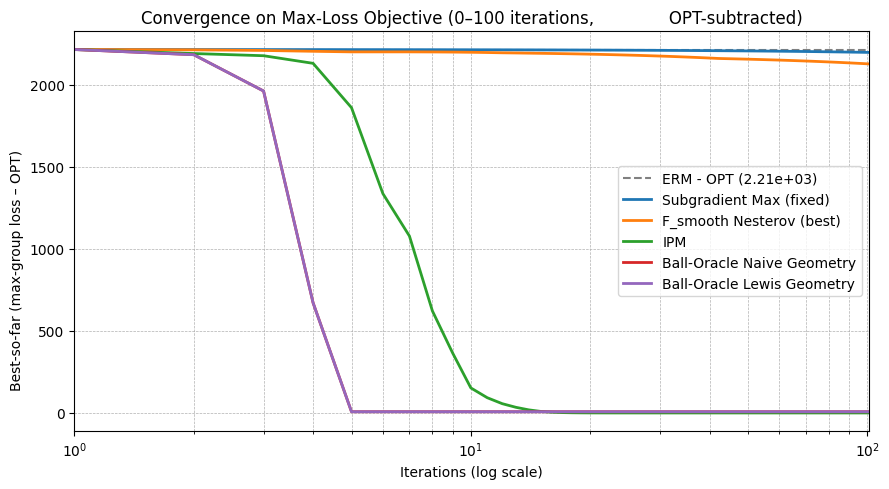
\includegraphics[width=\linewidth]{figures/Iterations.png}
        \caption{Suboptimality versus iteration count (log--log).}
    \end{subfigure}
    \hfill
    \begin{subfigure}{0.49\textwidth}
        \centering
        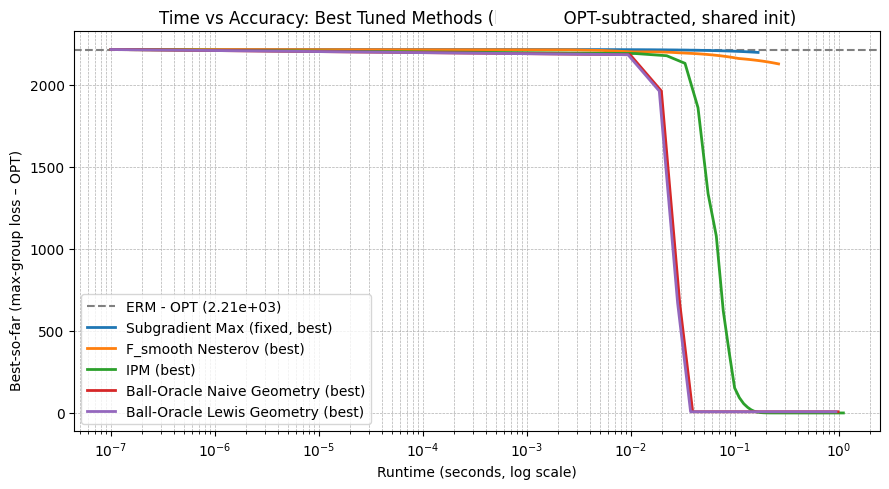
\includegraphics[width=\linewidth]{figures/Time.png}
        \caption{Suboptimality versus wall-clock time (seconds).}
    \end{subfigure}
    \caption{Comparison of first-order, interior-point, and ball-oracle methods on adversarial heterogeneous regression instances. All curves report the worst-group loss minus the optimal value computed via \texttt{CVXPY}.}
    \label{fig:iteration_runtime}
\end{figure}

% \begin{figure}[H]
%     \centering
%     \begin{subfigure}{\textwidth}
%         \centering
%         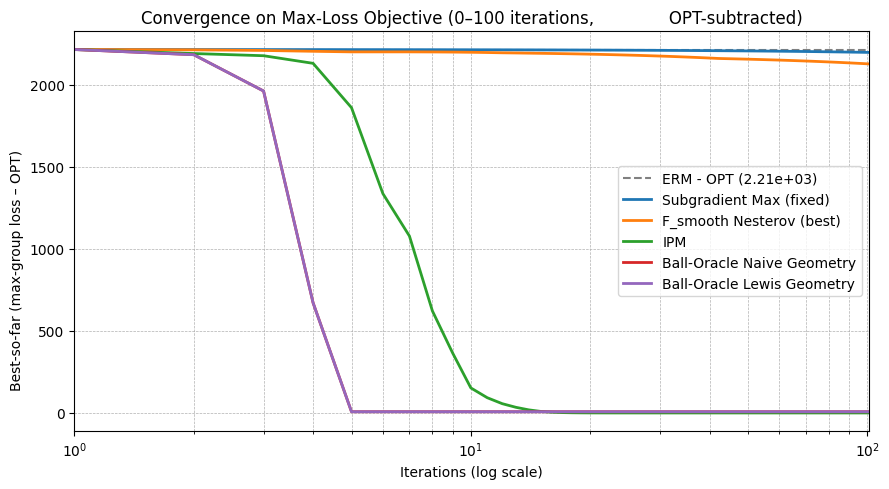
\includegraphics[width=\linewidth]{figures/Iterations.png}
%         \caption{Max-loss suboptimality versus iteration count (log scale on the x-axis).}
%     \end{subfigure}
%     % \hfill
%     \begin{subfigure}{\textwidth}
%         \centering
%         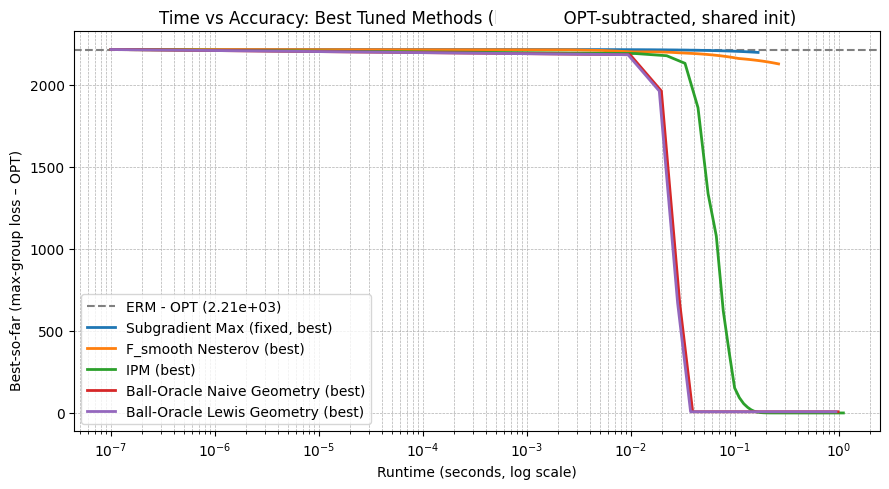
\includegraphics[width=\linewidth]{figures/Time.png}
%         \caption{Max-loss suboptimality versus runtime in seconds (log scale on the x-axis).}
%     \end{subfigure}
%     \caption{Comparison of first-order, interior-point, and ball-oracle methods on adversarial heterogeneous regression instances. All curves report the worst-group loss minus the optimal value computed via CVXPY.}
%     \label{fig:iteration_runtime}
% \end{figure}

\subsection{Real-world Experiment: ACS Income}
\label{app:acs}

To validate the computational behavior of our methods beyond synthetic instances, we evaluate them on a real-world group-structured regression task drawn from the American Community Survey (ACS), accessed through the \texttt{folktables} package~\citep{ding2021retiring}. The task is to predict log personal income from $d=10$ standardized demographic and employment features (age, education, occupation, hours worked, etc.) for employed US adults. We group the data by region of residence and use all $m=51$ regions (the $50$ states together with Puerto Rico), subsampling $200$ individuals per region for a total of $10{,}200$ samples. Each group loss $\ell_i$ is the mean squared prediction error on region $i$, and the objective is again the worst-group loss $F(\vx) = \max_{i\in[m]} \ell_i(\vx)$. This is a natural distributionally-robust setting: income distributions differ substantially across regions, so the model that minimizes the average error can perform poorly on individual states. All methods are warm-started at the empirical risk minimizer (ERM), and we compute the robust optimum $\opt$ with \texttt{CVXPY} as the reference value.

\paragraph{Convergence and runtime.} Our primary interest is computational: how quickly each method drives the worst-group suboptimality $F(\vx_t) - \opt$ to zero, both in outer iterations and in wall-clock time. \Cref{fig:acs_convergence} plots this gap against iteration count and against runtime, and \Cref{tab:acs_runtime} reports the iterations and wall-clock time each method needs to reach a relative suboptimality of $1\%$.

The two ball-oracle methods are the fastest on both axes. Starting from the warm start, each reaches the $1\%$ target in a \emph{single} outer iteration and in under $20$~ms of wall-clock time --- roughly $3\times$ faster than the interior-point method ($66$~ms, $8$ iterations) and the best-tuned smoothed Heavy-Ball method ($62$~ms, $47$ iterations). The interior-point method converges in a few iterations but incurs a higher per-iteration cost, whereas the smoothed first-order method requires an order-of-magnitude more iterations to reach the same accuracy. The subgradient method never reaches the $1\%$ target within the budget: it remains essentially pinned at the ERM gap (\Cref{fig:acs_convergence}). The Lewis-weight geometry is marginally faster than the Euclidean ball, consistent with the synthetic results. Overall, on a genuine $51$-group regression problem, the ball-oracle methods reach high-accuracy robust solutions fastest in both iteration count and wall-clock time.

\begin{figure}[t]
    \centering
    \begin{subfigure}{0.49\textwidth}
        \centering
        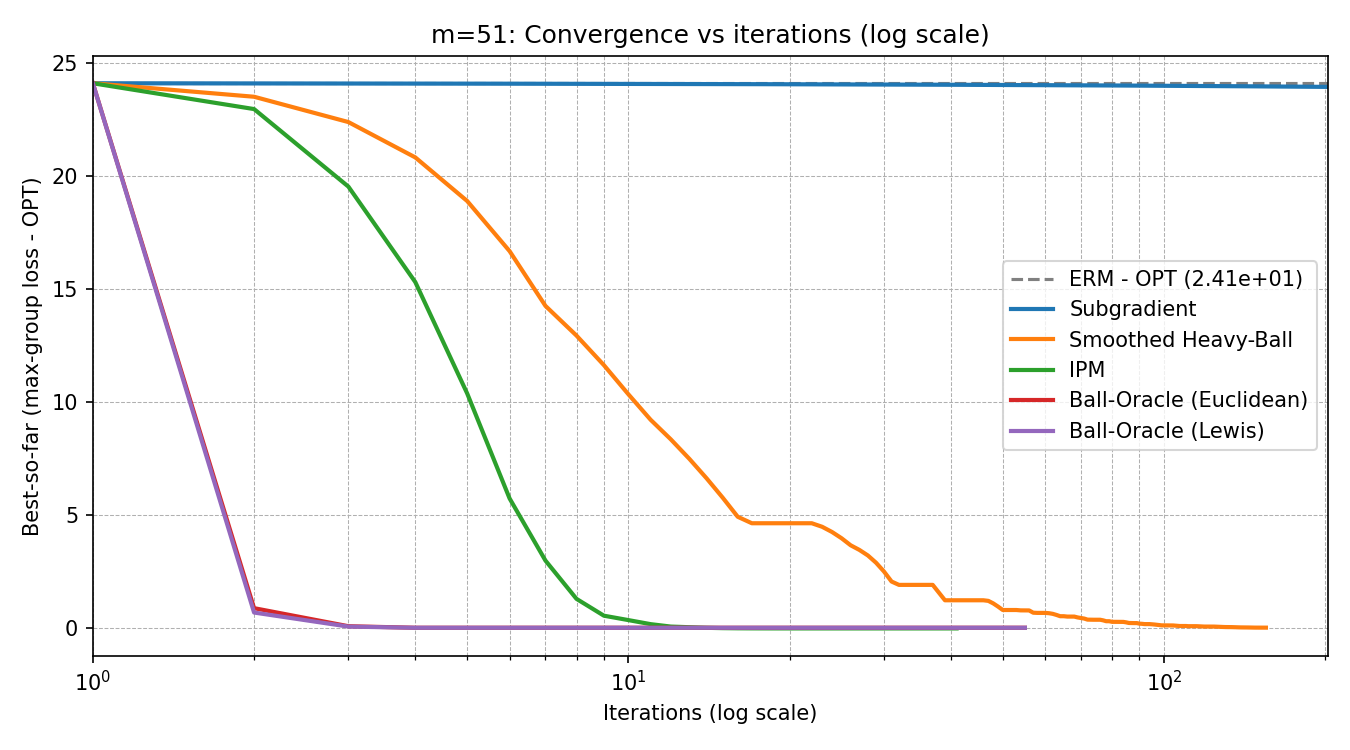
\includegraphics[width=\linewidth]{plots/acs_m51_iterations.png}
        \caption{Suboptimality versus iteration count (log--log).}
    \end{subfigure}
    \hfill
    \begin{subfigure}{0.49\textwidth}
        \centering
        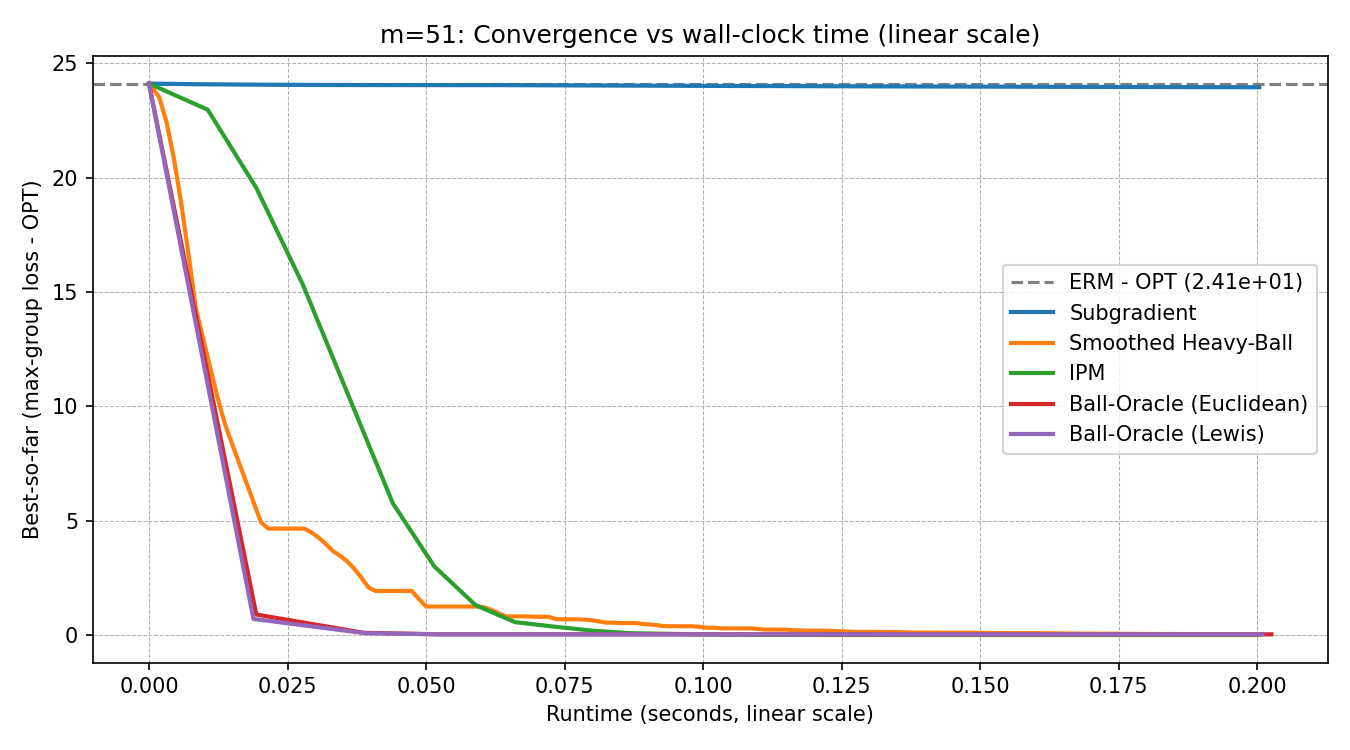
\includegraphics[width=\linewidth]{plots/acs_m51_time.png}
        \caption{Suboptimality versus wall-clock time (seconds).}
    \end{subfigure}
    \caption{Convergence on the ACS Income task ($m=51$ regions, $d=10$, $10{,}200$ samples). Each curve reports the best-so-far worst-group suboptimality $F(\vx_t) - \opt$; the dashed line marks the ERM gap. The ball-oracle methods reach the robust optimum in a single outer iteration and the least wall-clock time, while the subgradient method stalls at the ERM gap.}
    \label{fig:acs_convergence}
\end{figure}

\begin{table}[t]
    \centering
    \small
    \begin{tabular}{lrr}
        \toprule
        Method & Iterations to $1\%$ gap & Wall-clock time (s) \\
        \midrule
        Subgradient              & --- (not reached) & --- \\
        Smoothed Heavy-Ball      & 47 & 0.062 \\
        IPM                      &  8 & 0.066 \\
        Ball-Oracle (Euclidean)  &  1 & 0.019 \\
        Ball-Oracle (Lewis)      &  1 & 0.019 \\
        \bottomrule
    \end{tabular}
    \caption{Cost to reach a $1\%$ relative worst-group suboptimality on the ACS Income task ($m=51$). Iterations are each method's own natural outer iterations. The subgradient method does not reach the target within the iteration budget.}
    \label{tab:acs_runtime}
\end{table}

\paragraph{Statistical context.} For completeness, we note that the optimization gains correspond to meaningful redistribution of prediction accuracy across regions. The ERM solution attains the lowest \emph{average} error ($108.2$) but a large spread ($\sigma = 11.8$) and a worst-group loss of $138.1$, attained by California; other heavily penalized states are New York, Hawaii, Nevada, Florida, and New Jersey, all large or high-income regions on which a $10$-feature linear model underfits. The robust optimum instead nearly equalizes the group losses into a narrow band around $107$--$114$ (Max/Mean drops from $1.28$ to $1.02$), decreasing the loss on the previously neglected states (e.g.\ California by $24.3$~MSE) at a moderate cost on the homogeneous low-income states that ERM happened to fit well.